\documentclass[letterpaper,11pt]{article}

\author{Jacob Thomas Errington (260636023)}
\title{Assignment \#0\\Program analysis and transformations}
\date{13 September 2016}

\usepackage{hyperref}
\usepackage{graphicx}
\usepackage[margin=2.0cm]{geometry}

\begin{document}

\maketitle

\section{Background -- Compilers}

Last semester, I took the \textsc{COMP 520} course. The course primarily covers
the development and design of the frontend of a compiler throughout the project
component. The lectures covered some other aspects of programming language
development, such as runtime environments, the notion of bytecode interpreters,
garbage collection, and native code generation strategies.

In the project that I worked on last semester for \textsc{COMP 520},
\href{https://github.com/tsani/goto}{Goto}, my teammate and I implemented a
partial native code generator as well as a complete C++ code generator. Our
compiler furthermore offered a few other nice features, such as using the
standard error reporting format used in Vim, which allows integration with the
\texttt{:make} command, as well as reporting of multiple errors during
compilation (not a requirement of the project). We also strived to make our
error messages as informative as possible.

\section{Background -- Object-Oriented Programming}

Although I avoid OOP when I can, I have a fair amount of experience in it. Last
fall, I took the course \textsc{COMP 512} (Distributed Systems), in which there
is a term project component involving precisely a large prewritten codebase in
Java. I have also written a few simple games in C++ using OOP patterns. Also,
I have since February been working in backend web development in Python, which
although not essentially an OOP language, is used by my team in a reasonably
object-oriented way.

\section{Background -- \textsc{MATLAB}}

First time I've ever written MATLAB was for this assignment. I've used
Mathematica in the past, which I've concluded is similar in some regards
(target audience, lots of built-ins, nice plotting) but different in others
(pretty much everything else).

I will have to admit that I did not use MATLAB proper to complete the
assignment; I used Octave. The reason being that sometimes, I am a bad student,
and leave this sort of thing to the last minute, only to discover that for some
strange reason I am unable to SSH into most of the Trottier lab machines and
that the ones I can access don't have matlab installed.

Anyway, I adapted the example of computing a bunch of sines given in the MATLAB
documentation regarding vectorization. I modified it somewhat. I collected the
data in MATLAB, wrote it to a file, and made chart \ref{fig:data} in Python.

\begin{figure}[ht]
    \centering
    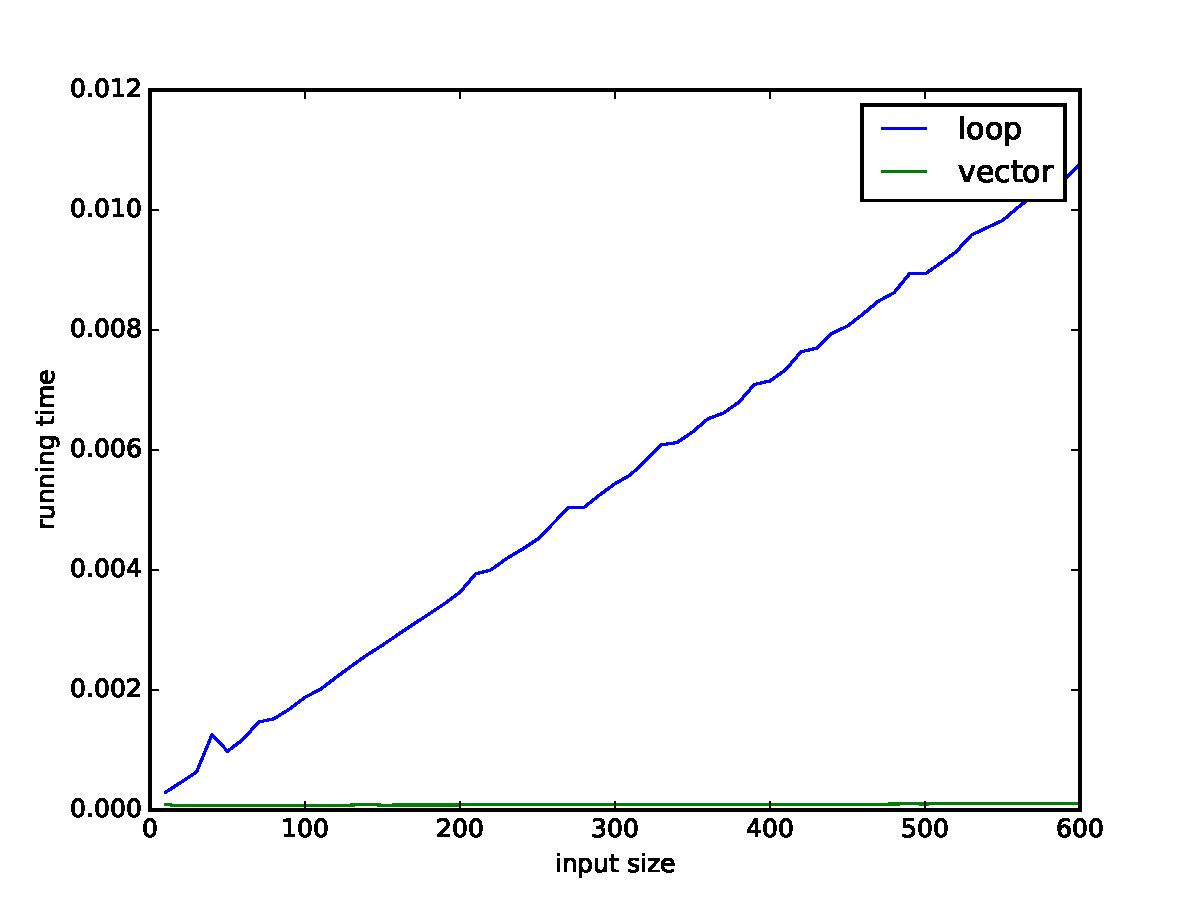
\includegraphics[width=0.8\textwidth]{fig.pdf}
    \label{fig:data}
\end{figure}

The vector version of the execution is visibly flat, whereas the loop
version's running time is linear in comparison. Of course, the vector version
is \emph{flat} because that is impossible. The data I collected is attached,
and one can see that the running time does increase overall. The vectorized
version, due to the use of the built-in looping capability of the vectorized
\texttt{sin} function, is presumably performing the loop far more closely to
the machine, perhaps because the Octave interpreter calls out to a routine in C
to perform that loop. For instance, I know that NumPy achieves its speeds
precisely due to tricks like that. On the other hand, the interpreter is unable
to optimize my handwritten loop and consequently executes it instruction by
instruction, resulting in a much greater constant factor in the linear growth
of the loop-based implementation.

\end{document}
